\begin{document}

\begin{frame} 
	\frametitle{\parbox{1.03\linewidth}{\centering{\fontsize{17pt}{10pt}\color{white}\selectfont Universidade Estadual de Maringá}}}
	
	\title{Experimento x\\
		\small }
	
	\ifbool{MODE_DEV}{}{\logo{
\includegraphics[width=1.6cm,height=1.4cm]{img/uem2.png}}}
	\author[]{
		Tiririca\\%
		Einsten da silva \\
		José Cristo\\
		Compadre Washington  \\%- RA:PG47547}
	}
	\institute{\color{black}
		Prof.\textordfeminine Obama \\
		Mestrado em Ciência da Computação \\
	Departamento de Informática}									 
										
	\titlepage
										
\end{frame}
\begin{frame}{Tópicos}
	\tableofcontents[sections={1-10}] 
\end{frame}
%\begin{frame}{Sumário}
%   \tableofcontents[sections={7-}] 
%\end{frame}
 

% Uncomment these lines for an automatically generated outline.
%\begin{frame}{Outline}
%  \tableofcontents
%\end{frame}


\section{Introdução}



\begin{frame}{Introdução}
	
	\begin{itemize}
	\item De acordo com \citet{Vieira2006}, blabla 
	\pause
	\item As LLC sao tipo 2 da hierarquia de Chomsky.
	\pause
	\item Bombeamento para LLC.
	\end{itemize} 
	 
\end{frame}

\begin{frame}{Introdução}
\prompt{O que é caviar?}{Não sei. Nunca vi. Só ouço falar}
\end{frame}

\input{text/part2}
\input{text/part3}
\input{text/part4}



\section{Finalização} 



\begin{frame}{Agradecimento}
		
	\begin{center}
		\centering
			 
		% \setfont{calligra}{Obrigado} 
		\hspace*{-1cm}\scalebox{3}{
			{\Huge\textcalligra{Obrigado}}}
	\end{center}
	\centering
	%	\begin{figure}
	%		\centering
	%		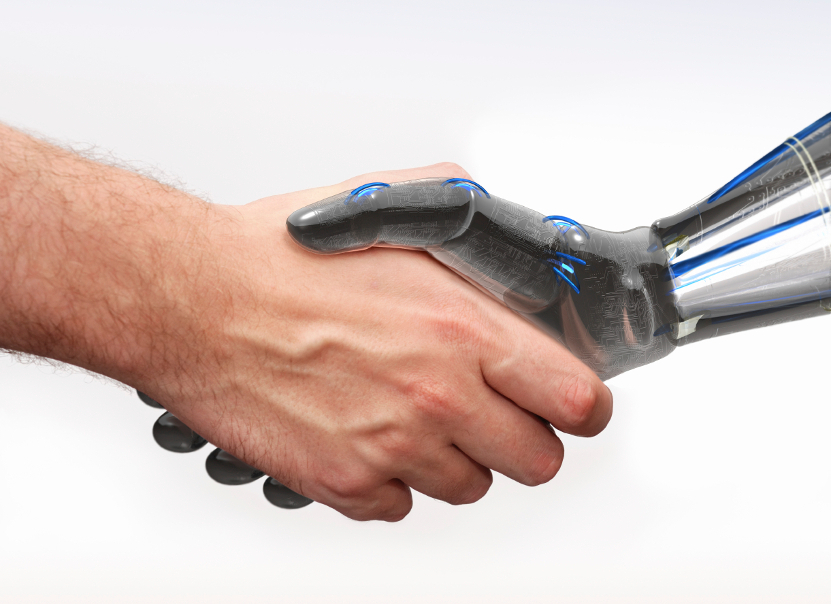
\includegraphics[width=7cm,keepaspectratio=true]{img/hand.jpg}
	%	\end{figure}
	
\end{frame}

\begin{frame}{Perguntas}
	\begin{figure}
		\centering
		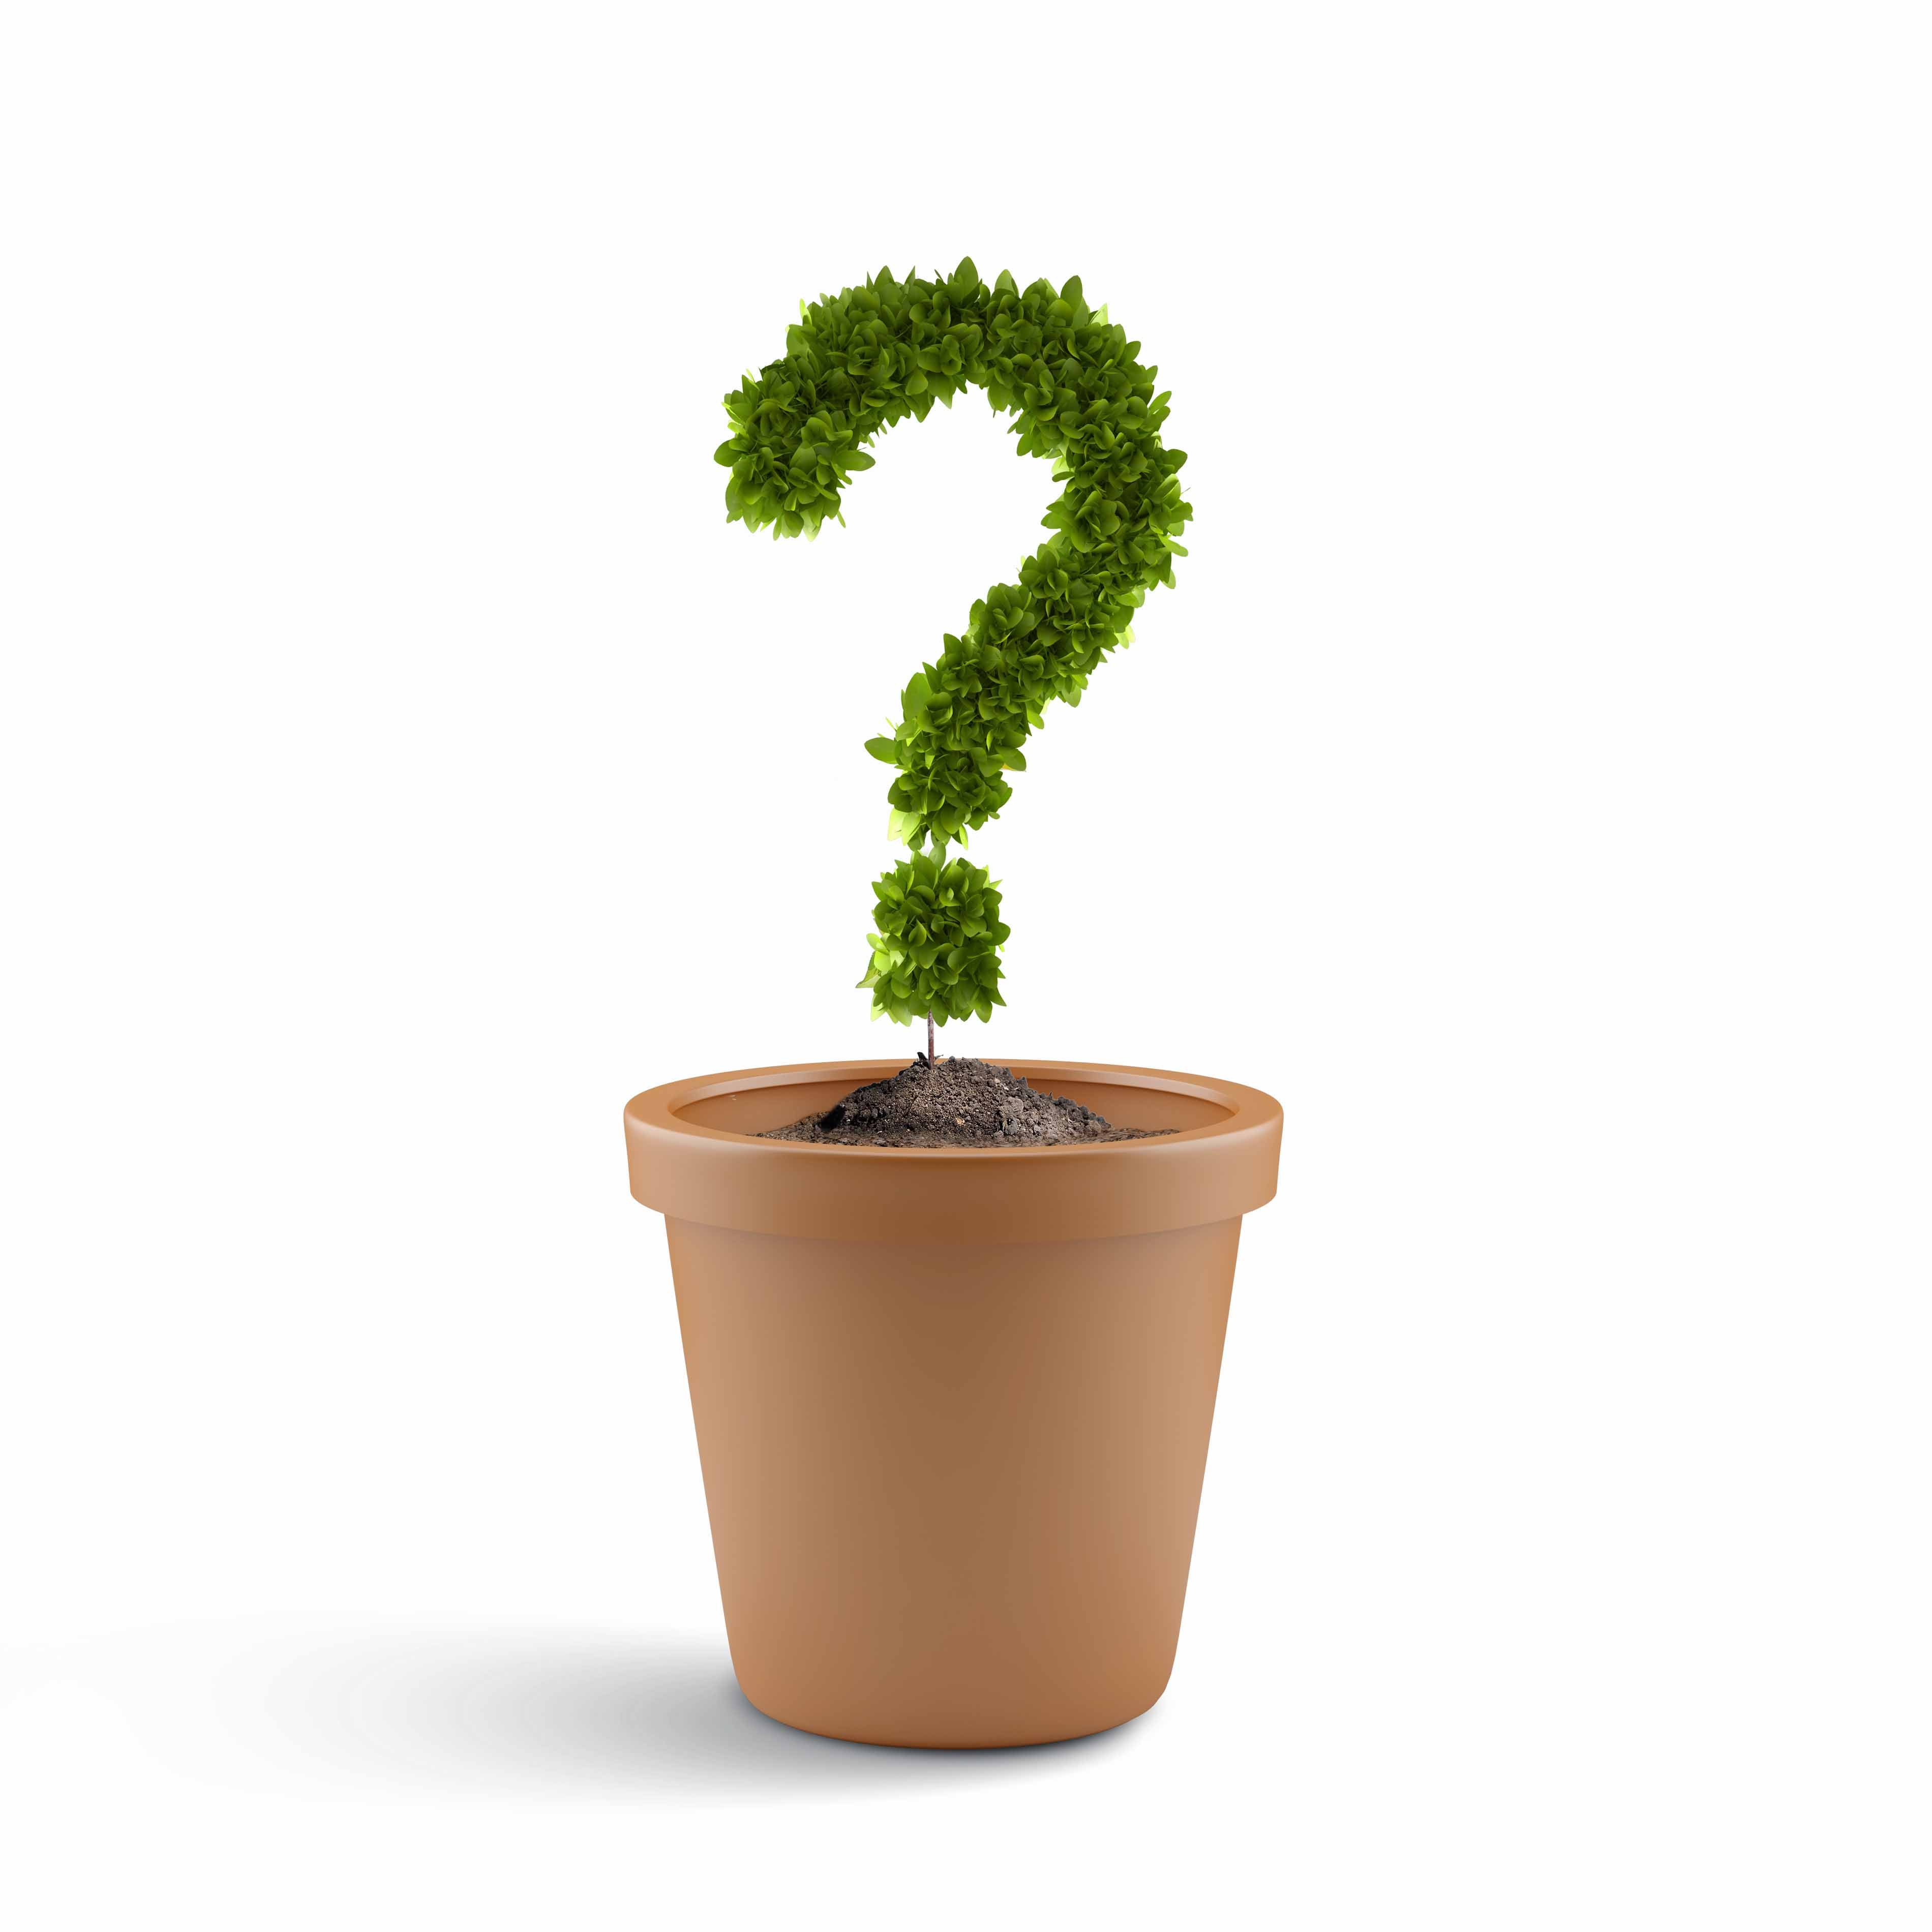
\includegraphics[width=7cm,keepaspectratio=true]{img/ask.jpg}
	\end{figure}
\end{frame}

\appendix
\begin{frame}[allowframebreaks]{Referências}
        %       \bibliographystyle{abbrvnat}
        \bibliography{text/references}
\end{frame}





\end{document}

